\documentclass{article} % For LaTeX2e
\usepackage{nips15submit_e,times}
\usepackage{hyperref}
\usepackage{url}
\usepackage{amssymb}
\usepackage{amsmath}
\usepackage{booktabs}
\usepackage{graphicx}

%\documentstyle[nips14submit_09,times,art10]{article} % For LaTeX 2.09

\title{Feed-Forward Networks with Attention Can Solve Some Long-Term Memory Problems}


\author{
Colin Raffel\\
LabROSA, Columbia University\\
\texttt{craffel@gmail.com}
\And
Daniel P.~W.~Ellis\\
LabROSA, Columbia University\\
\texttt{dpwe@ee.columbia.edu}
}

\newcommand{\fix}{\marginpar{FIX}}
\newcommand{\new}{\marginpar{NEW}}

\nipsfinalcopy % Uncomment for camera-ready version

\begin{document}

\maketitle

\begin{abstract}
Recurrent neural networks (RNNs) have proven to be powerful models in problems where variable-length sequences are projected into a fixed-dimensional embedded space.
Recently, RNNs have been augmented with ``attention'' mechanisms which allow the network to focus on different parts of an input sequence when computing their output.
We propose a simplified model of attention which is applicable to feed-forward neural networks and demonstrate that it can solve some long-term memory problems (specifically, those where temporal order doesn't matter).
In fact, we show empirically that our model can solve these problems for sequence lengths which are both longer and more widely varying than the best results attained with RNNs.
\end{abstract}

\section{Models for Sequential Data}

Many problems in machine learning are best formulated using sequential data, i.e.\ data where a given observation may be dependent on previous observations.
Such problems can be coarsely classified as sequence transduction (producing a new sequence given an input sequence), sequence embedding (producing a single label, value, or vector from an entire sequence), or sequence generation (producing a sequence from no input).
Appropriate models for these tasks must be able to capture temporal dependencies in sequences, potentially of arbitrary length.

\subsection{Recurrent Neural Networks}

One such class of models are recurrent neural networks (RNNs), which can be considered a learnable function $f$ whose output $h_t = f(x_t, h_{t - 1})$ at time $t$ depends on input $x_t$ and the previous state $h_{t - 1}$.
In the supervised setting, the parameters of $f$ are optimized with respect to a loss function which measures $f$'s performance.
A common approach is to use backpropagation through time \cite{werbos1990backpropagation}, which ``unrolls'' the RNN over time steps to compute the gradient of the parameters of $f$ with respect to the loss.
Because the same function $f$ is applied repeatedly over time, this gradient can easily explode or vanish \cite{pascanu2012difficulty,hochreiter1997long,bengio1994learning}.
The use of gating architectures \cite{hochreiter1997long,cho2014learning}, sophisticated optimization techniques \cite{martens2011learning,sutskever2013importance}, gradient clipping \cite{pascanu2012difficulty,graves2013generating}, and/or careful initialization \cite{sutskever2013importance,jaegar2012long,mikolov2014learning,le2015simple} can help mitigate this issue and has facilitated the success of RNNs in a variety of fields (see e.g.\ \cite{graves2012supervised,cho2015describing} for an overview).
However, these approaches don't \textit{solve} the problem of vanishing and exploding gradients, and as a result RNNs are in practice typically only applied in tasks where sequential dependencies span at most hundreds of time steps \cite{martens2011learning,sutskever2013importance,le2015simple,hochreiter1997long}.
Very long sequences can also make training computationally inefficient due to the fact that RNNs must be evaluated sequentially and cannot be fully parallelized.

\subsection{Attention}

A recently proposed method for easier modeling of long-term dependencies is ``attention''.
Attention mechanisms allow for a more direct dependence between the state of the model at different points in time.
Following the definition from \cite{bahdanau2014neural}, given a model which produces a hidden state $h_t$ at each time step, attention-based models first compute a ``context'' vector $c_t$ as the weighted mean of the state sequence $h$ by
$$
c_t = \sum_{j = 1}^T \alpha_{tj} h_j
$$
where $T$ is the total number of time steps in the input sequence and $\alpha_{tj}$ is a weight computed at each time step $t$ for each state $h_j$.
These context vectors are then used to compute a new state sequence $s$, where $s_t$ depends on $s_{t - 1}$, $c_t$ and, for sequence prediction, the model's output at $t - 1$.
The weightings $\alpha_{ij}$ are then computed by
\begin{align*}
e_{tj} &= a(s_{t - 1}, h_j)\\
\alpha_{tj} &= \frac{\exp(e_{tj})}{\sum_{k = 1}^T \exp(e_{tk})}
\end{align*}
where $a$ is a learned function which can be thought of as computing a scalar importance value for $h_j$ given the value of $h_j$ and the previous state $s_{t - 1}$.
This formulation allows the new state sequence $s$ to have more direct access to the entire state sequence $h$.
Attention-based RNNs have proven effective in a variety of sequence transduction tasks \cite{bahdanau2014neural,cho2015describing}.
RNNs with attention can be seen as analogous to the recently proposed Memory Network \cite{weston2014memory,sukhbaatar2015end} and Neural Turing Machine \cite{graves2014neural} models.

\subsection{Feed-Forward Attention}

A straightforward simplification to the attention mechanism described above which would allow it to be applied to sequence embedding tasks could be formulated as follows:
Instead of a sequence of context vectors, we produce a single context vector $c$ as
\begin{align}
\begin{split}
\label{eq:ffattention}
e_t &= a(h_t)\\
\alpha_t &= \frac{\exp(e_t)}{\sum_{k = 1}^T \exp(e_k)}\\
c &= \sum_{t = 1}^T \alpha_t h_t
\end{split}
\end{align}
As before, $a$ is a learnable function, but it now only depends on $h_t$.
In this formulation, attention can be seen as producing a fixed-length embedding $c$ of the input sequence by computing an adaptive weighted average of the state sequence $h$.  A schematic of this form of attention is shown in Figure \ref{fig:schematic}.

\begin{figure}
  \centering
  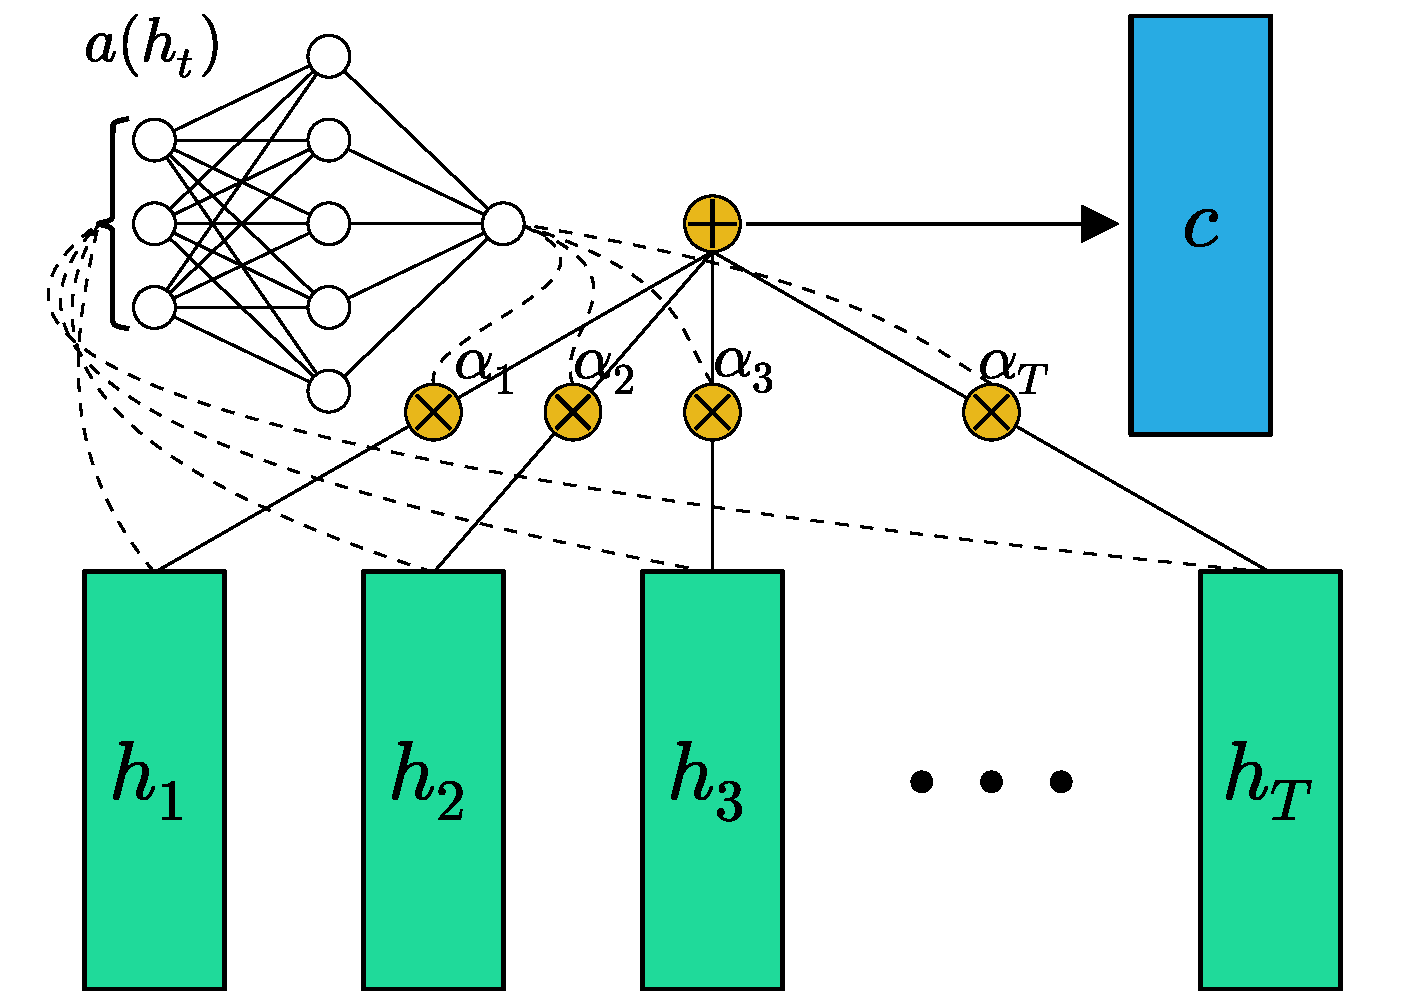
\includegraphics[width=.8\textwidth]{schematic.pdf}
  \caption{Schematic of our proposed ``feedforward'' attention mechanism (cf.\ \cite{cho2015introduction} Figure 1).  Vectors in the hidden state sequence $h_t$ are fed into the learnable function $a(h_t)$ to produce a probability vector $\alpha$.  The vector $c$ is computed as a weighted average of $h_t$, with weighting given by $\alpha$.}
  \label{fig:schematic}
\end{figure}


A consequence of using an attention mechanism is that the context vector $c$ can model temporal dependencies because attention performs integration over time.
It follows that by using this simplified form of attention, a model could perform sequence embedding even if the calculation of $h_t$ was feed-forward, i.e.\ $h_t = f(x_t)$.
Using a feed-forward $f$ could also result in large efficiency gains as the computation could be completely parallelized.
While using a feed-forward model for sequential modeling sacrifices the ability to solve some problems, we show that for certain tasks, feed-forward networks with attention can perform arbitrary-length sequence embedding as effectively than RNNs.

We note here that feed-forward models without attention can be used for sequence embedding when the sequence length $T$ is fixed, but when $T$ varies across sequences, some form of temporal integration is necessary.
An obvious straightforward choice, which can be seen as an extreme oversimplification of attention, would be to compute $c$ as the unweighted average of the state sequence $h_t$, i.e.
\begin{equation}
\label{eq:unweighted}
c = \frac{1}{T}\sum_{t = 1}^T h_t
\end{equation}
We will also explore the effectiveness of this approach for sequence embedding.

\section{Toy Long-Term Memory Problems}

A common way to measure the long-term memory capabilities of a given model is to test it on the synthetic problems originally proposed in \cite{hochreiter1997long}.
In this paper, we will focus on the ``addition'' and ``multiplication'' problems, which can be summarized as follows:
The input is a two dimensional sequence, where one dimension is a random sequence sampled uniformly from $[0, 1]$ and the other dimension is a ``mask'' sequence.
At two time steps, one in the first ten sequence steps and one before the sequence's midpoint, the ``mask'' signal is 1; at the first and last time step it is -1; and at all other time steps it is 0.
The goal is to perform addition or multiplication on the two values in the noise dimension which co-occur with the 1s in the mask dimension, which is meant to require that a model be able to store the correct values for the duration of the sequence.
A sequence is considered correctly processed if the absolute difference between the predicted and target values is less than $.04$.
Slight variants of these tasks have also been used \cite{sutskever2013importance,le2015simple,jaegar2012long,martens2011learning}, but we will follow the original definition from \cite{hochreiter1997long}.
These two tasks are only a subset of the synthetic long-term memory problems which have been proposed; we focus on them here because they are the most commonly used and discuss the applicability of feed-forward attention on the remaining problems in Section \ref{sec:limitations}.

\subsection{Model Details}

For all experiments, we used the following model:
First, the state $h_t$ was computed from the input at each time step $x_t$ by 
$$
h_t = \max(W_{xh}x_t + b_{xh}, 0.01)
$$
where $W_{xh} \in \mathbb{R}^{D \times 2}, b_{xh} \in \mathbb{R}^D$.
We tested models where the context vector $c$ was then computed either as in Equation \ref{eq:ffattention}, with 
$$
a(h_t) =\tanh(W_{hc}h_t + b_{hc})
$$
where $W_{hc} \in \mathbb{R}^{1 \times D}, b_{hc} \in \mathbb{R}$, or simply as the unweighted mean of $h$ as in Equation \ref{eq:unweighted}.
We then computed an intermediate vector 
$$
s = \max(W_{cs}c + b_{cs}, 0.01)
$$
where $W_{cs} \in \mathbb{R}^{D \times D}, b \in \mathbb{R}^D$ from which the output was computed as
$$
y = \max(W_{sy}s + b_{sy}, 0.01)
$$
where $W_{sy} \in \mathbb{R}^{1 \times D}$, $b_{sy} \in \mathbb{R}$.
The ``leaky rectifier'' nonlinearity $\textrm{LReLU}(x) = \max(x, .01)$ was proposed in \cite{maas2013rectifier}; we found that it improved early convergence so we used it in all of our models.
For all experiments, we set $D = 100$.

We used the squared error of the output $y$ against the target value for each sequence as an objective.
Parameters were optimized using ``adam'', a recently proposed stochastic optimization technique \cite{kingma2014adam}, with the optimization hyperparameters $\beta_1$ and $\beta_2$ set to the values suggested in \cite{kingma2014adam} (.9 and .999 respectively).
$W_{xh}, W_{hc}, W_{cs}, W_{so}$ were all initialized using He's method \cite{he2015delving} and $b_{xh}, b_{hc}, b_{cs}, b_{so}$ were all initialized to 0 vectors.
We trained on mini-batches of 100 sequences and computed the accuracy on a held-out test set of 1000 sequences every epoch, defined as 1000 parameter updates.
We stopped training when either 100\% accuracy was attained on the test set, or after 100 epochs.
All networks were implemented using Lasagne \cite{dieleman2015lasagne}, which is built on top of Theano \cite{bastien2012theano,bergstra2010theano}.

\begin{table}
  \centering
  \begin{tabular}{r c c c c c c}
    \toprule
    \multicolumn{7}{c}{\textbf{Addition}} \\
    $T_0$ & 50 & 100 & 500 & 1000 & 5000 & 10000 \\
    \cmidrule(r){2-7}
    Attention & 1 & 1 & 1 & 1 & 2 & 3 \\
    Unweighted & 1 & 1 & 1 & 2 & 8 & 17 \\
    \midrule
    \multicolumn{7}{c}{\textbf{Multiplication}} \\
    $T_0$ & 50 & 100 & 500 & 1000 & 5000 & 10000 \\
    \cmidrule(r){2-7}
    Attention & 1 & 2 & 4 & 2 & 15 & 6 \\
    Unweighted & 2 & 2 & 8 & 33 & \textcolor{gray}{89.8\%} & \textcolor{gray}{80.8\%} \\
    \bottomrule
  \end{tabular}
  \caption{Number of epochs required to achieve perfect accuracy, or accuracy after 100 epochs (greyed-out values), for the experiment described in Section \ref{sec:fixed}.}
  \label{tab:fixed}
\end{table}
\setlength{\textfloatsep}{14pt}

\subsection{Fixed-Length Experiment}
\label{sec:fixed}

Traditionally, the sequence lengths tested in each task vary uniformly between $[T_0, 1.1T_0]$ for different values of $T_0$.
As $T_0$ increases, the model must be able to handle longer term dependencies.
The largest value of $T_0$ for which high accuracy was attained on a held-out test set varies across models, tasks and papers; as a rough overview \cite{sutskever2013importance} uses $T_0 = 80$, \cite{le2015simple,martens2011learning} achieve success for $T_0 \le 250$, and \cite{jaegar2012long,hochreiter1997long} achieve success for $T_0 \le 1000$ except \cite{jaegar2012long} solves the addition task for $T_0 = 10000$.
We therefore tested our proposed feed-forward attention models for $T_0 \in \{50, 100, 500, 1000, 5000, 10000\}$.
The required number of epochs or accuracy after 100 epochs for each task, sequence length, and temporal integration method (adaptively weighted attention or unweighted mean) is shown in Table \ref{tab:fixed}.
For fair comparison, we report the best result achieved using any learning rate in $\{.0003, .001, .003, .01\}$.
From these results, it's clear that the feed-forward attention model can solve these long-term memory problems with comparable, and sometimes longer, sequence lengths than have been achieved with RNNs.
Our model is also extremely efficient: Processing one epoch of 100,000 sequences with $T_0 = 5000$ took about two minutes using an NVIDIA GTX 980 Ti GPU.
In addition, there is a clear benefit to using the attention mechanism of Equation \ref{eq:ffattention} instead of a simple unweighted average over time, which only incurs a marginal increase in parameters.

\subsection{Variable-length Experiment}

Because the range of sequence lengths $[T_0, 1.1T_0]$ is small compared to the range of $T_0$ values we evaluated, we further tested whether it was possible to train a single model which could cope with sequences with highly varying lengths.
To our knowledge, such an experiment has not been conducted with RNNs.
We trained models of the same architecture as used in the previous experiment on sequences with lengths varying uniformly from 50 to 10000 time steps.
Using the attention mechanism of Equation \ref{eq:ffattention}, on held-out test sets of 1000 sequences, our model achieved 99.9\% accuracy on the addition task and 99.4\% on the multiplication task.
This suggests that a single feed-forward network with attention can simultaneously model both short-term and long-term dependencies, with a marginal decrease in accuracy.
Using an unweighted average over time, we were only able to achieve accuracies of 77.4\% and 55.5\% on the variable-length addition and multiplication tasks, respectively.

\section{Discussion}
\label{sec:limitations}

A clear limitation of our proposed model is that it will fail on any task where temporal order matters because computing an average over time discards temporal information.
For example, on the two-symbol temporal order task \cite{hochreiter1997long} where a sequence must be classified in terms of whether two symbols $X$ and $Y$ appear in the order $X, X$; $Y, Y$; $X, Y$; or $Y, X$, our model can differentiate between the $X, X$ and $Y, Y$ cases perfectly but cannot differentiate between the $X, Y$ and $Y, X$ cases at all.
Nevertheless, we submit that for some real-world tasks involving sequential data, temporal order is substantially less important than being able to handle very long sequences.
In these cases, our results suggest that a completely feed-forward attention-based network could be substantially more efficient than recurrent models.
Further investigation on real-world problems is warranted; for interested researchers, all of the code used in this experiment is available online.\footnote{\href{https://github.com/craffel/sequence-embedding/tree/master/toy_problems}{\texttt{https://github.com/craffel/sequence-embedding/tree/master/toy\char`_problems}}}

\bibliographystyle{unsrt}
\small
\bibliography{refs}

\end{document}
